\documentclass[11pt,a4paper]{article}
\usepackage[T1]{fontenc}
\usepackage{lmodern}
\input{glyphtounicode}
\pdfgentounicode=1
\usepackage{amsmath,amssymb,amsthm}
\usepackage{graphicx}
\usepackage{booktabs}
\usepackage{microtype}
\usepackage{geometry}
\usepackage{doi}
\usepackage{hyperref}
\geometry{margin=2.5cm}

\hypersetup{
  pdftitle={Asymptotic Calibration of the BFS Window and Effective Dimension of the Admissible Trajectory},
  pdfauthor={J\'er\^ome Beau},
  pdfsubject={Finite-size window calibration and effective covariance dimension in spectral admissibility},
  pdfkeywords={spectral admissibility, BFS window depth, Weil representation, Heisenberg graphs,
    covariance operator, effective dimension, Born--Infeld saturation}
}

\newtheorem{theorem}{Theorem}[section]
\newtheorem{proposition}[theorem]{Proposition}
\newtheorem{lemma}[theorem]{Lemma}
\newtheorem{corollary}[theorem]{Corollary}
\theoremstyle{definition}
\newtheorem{definition}[theorem]{Definition}
\newtheorem{remark}[theorem]{Remark}

\title{Asymptotic Calibration of the BFS Window\\
and Effective Dimension of the Admissible Trajectory\\[4pt]
\large O28 --- Spectral Admissibility Sub-programme}
\author{J\'{e}r\^{o}me Beau\\
\small Independent Researcher\\
\small \texttt{jerome.beau@cosmochrony.org}}
\date{2026}

\begin{document}
  \maketitle

  \begin{abstract}
    The O25 programme identified the ratio $n_1(q)/q$ as the central open
    asymptotic variable controlling the finite-size drift of $\bar{\delta}_{\mathrm{pair}}(q)$,
    and O26--O27 identified the effective dimension
    $r_{\mathrm{eff}} = d_\rho^2$ of the per-pair covariance operator in $\mathrm{End}(V_\rho)$
    as the key falsifiability criterion for the representation-theoretic identification.
    The present paper reports two analyses built from the Q5a-O5 checkpoints and their documented
    prime-range extensions.
    First, we extract $n_1(q)$ from the auto-calibrated fitting windows and fit
    $n_1(q) = \hat{\alpha}\,q + \hat{\beta}$ by ordinary least squares, obtaining
    $\hat{\alpha} \approx 0.053$ with $R^2 \approx 0.879$ over $q \le 211$.
    Extending the window-depth measurement out of sample to $q \in \{307, 401, 503, 601\}$ makes
    this calibrated linear extrapolation fail (it overpredicts $n_1$ by up to $+88\%$).
    The exact law is established in the companion Critical Coverage note: $n_1(q) \to 22$ in
    probability for five independently and uniformly sampled generic blocks, with critical
    coverage $x_1(q) = |B_{n_1}|/q^2 \asymp q^{-2}$; the measured decrease of $n_1(q)/q$ belongs
    to the transitional resonance regime of that law.
    The declared finite-size adjustment
    $\delta_{\mathrm{corr}}(q) = \bar{\delta}_{\mathrm{pair}}(q) - \eta\log q/\log n_1(q)$
    lies in $[7.4, 10.6]$ for all $q \in \{29, 61, 101, 151, 211\}$; O14 establishes that this term
    does not correct the intra-$q$ fitted exponent, so the stability is a diagnostic and not a
    corrected capacity exponent.
    Second, using the per-block Weil vector projections $\pi_c(v)$ stored in the Q5a-O5
    checkpoints, we perform the formal effective-dimension computation of O26 Criterion~5.4
    in $\mathrm{End}(H_{\mathrm{eff}})$, where $H_{\mathrm{eff}} = \mathbb{C}^3$ is the
    admissible projection space ($\mathrm{HEFF\_DIM} = 3$, consistent with the supplied
    selection rule $\Sigma_c(n_3) = 3$ of O23).
    Over the samples of the present perimeter, the covariance $\mathcal{C}_c$ has $1\%$ threshold
    rank $r_{\mathrm{eff}}^{1\%} = 3$ for every conjugate pair at $q \in \{61, 101, 151\}$, with
    normalised resolved spectrum
    $[\lambda_1 : \lambda_2 : \lambda_3] = [1 : \tfrac{1}{2} : \tfrac{1}{2}]$.
    This is a finite-data value of the stated protocol and not an invariant: the extended
    recomputation of O29 finds rank three modal, at $32/50$ pairs for $q = 101$ and $103/105$ for
    $q = 211$.
    These three resolved modes fill $H_{\mathrm{eff}}$ at the stated threshold.
    The gap from the spin-$\tfrac{1}{2}$ prediction $d_\rho^2 = 4$ reflects that
    $H_{\mathrm{eff}} \neq V_\rho$, and stays open.
    O29 audits what the measurement identifies: the projected-coordinate relation
    $\pi_{q-c}(v) = \overline{\pi_c(v)}$ is motivated by the Weil-block identity
    $\rho_{q-c} = \bar\rho_c$ without following from it, the finite-precision diagnostics are
    compatible with an adjoint reading of $H_{\mathrm{eff}}$ without deriving that carrier, and
    $V_\rho$ is supplied elsewhere rather than recovered from these data.
    Interpretively, the combined result separates a finite-$q$ calibration diagnostic from its
    proved asymptotic law, and leaves the spin-$\tfrac{1}{2}$ dimension unmeasured by the
    conjugate-pair covariance.
  \end{abstract}

  \paragraph{Keywords.}
    spectral admissibility; BFS window depth; pair observable; Weil representation; Heisenberg graphs; capacity
    exponent; normalisation correction; covariance operator; effective dimension; admissible trajectory; Born--Infeld
    saturation

    \clearpage
    \tableofcontents

    \clearpage

  \section{Position of the Problem}

  \subsection{What O25--O27 established}

    Paper O25~\cite{Beau2026a29} established three results for the pair observable
    $\sigma_{\mathrm{pair}}(n) = \sigma_c(n)\,\sigma_{q-c}(n)$ on
    $\mathrm{Heis}_3(\mathbb{Z}/q\mathbb{Z})$:
    (i) the inter-pair standard deviation of $\delta_{\mathrm{pair}}$ decreases monotonically
    from $0.54$ at $q = 29$ to $0.11$ at $q = 211$, strengthening the evidence that
    $\delta_{\mathrm{pair}}$ is a structural invariant of the Weil representation;
    (ii) empirical fits carry no asymptotic meaning because the leading finite-size correction
    $\eta\log q/\log n_1(q) \approx 1$ is itself $q$-dependent;
    (iii) after the finite-size adjustment $\eta\log q/\log n_1(q)$ of~\eqref{eq:dcorr}, the
    adjusted values fall within the window $[7.4, 10.6]$.
    O25 identified the ratio $n_1(q)/q$ as the central open direction.

    Paper O26~\cite{Beau2026a30} established a dictionary between conjugate Weil blocks and
    rank-one matrix coefficients in a representation space, and formulated a hierarchy of
    identifications (Levels~I--III).
    Test~4 of O26 (Criterion~5.4) provides the key falsifiability criterion: the effective
    dimension $r_{\mathrm{eff}}$ of the per-pair covariance operator
    \begin{equation}
      \mathcal{C}_c = \frac{1}{N}
      \sum_{n=n_0}^{n_1}
      \operatorname{vec}(\widetilde{M}^f_n)\,\operatorname{vec}(\widetilde{M}^f_n)^\dagger
      \label{eq:covariance}
    \end{equation}
    in $\operatorname{End}(V_\rho)$ should equal $d_\rho^2 = 4$ for the spin-$\tfrac{1}{2}$
    sector candidate.

    Paper O27~\cite{Beau2026a31} shows that any morphism satisfying the three structural
    constraints factors uniquely through the admissibility quotient, and exhibits the canonical
    representation action $\rho \colon \mathfrak{su}(2) \to \operatorname{End}(V_\rho)$ under two
    premises: the identification of the admissible image with the neutral traceless sector,
    $\operatorname{Im}\Pi_{\mathrm{adm}} = \mathrm{Ntrl}$, which is assumed and derived nowhere,
    and the spinor carrier supplied conditionally by O23.
    The vector lift asked for in O26 Hypothesis~4.4 remains open.
    The full implication chain
    \[
      \text{emergence} \Rightarrow \text{non-injectivity}~\cite{Beau2026l}
      \Rightarrow \text{pair structure} \Rightarrow \text{quadratic form}
      \Rightarrow \mathfrak{su}(2)
    \]
    is thereby carried at the structural level, with arrows of unequal type.
    What the covariance structure of the admissible trajectory measures is the object of the
    present paper (Part~B) and of the audit in O29~\cite{Beau2026a33}; no irreducible sector is
    identified there.

  \subsection{Scope of O28}

    O28 addresses the two numerical questions left open after O25--O27:
    \begin{enumerate}
      \item \textbf{Part~A}: determine the asymptotic behaviour of the auto-calibrated window depth
      $n_1(q)$, test the linear scaling hypothesis suggested by the initial calibration range, and
      reassess $\delta_{\mathrm{corr}}(q)$ using the measured window depths.
      \item \textbf{Part~B}: perform the formal effective-dimension computation of
      O26 Criterion~5.4 using the per-block Weil vector projections $\pi_c(v) \in H_{\mathrm{eff}}$
      stored in the Q5a-O5 checkpoints, and determine what the covariance structure of
      $\mathcal{C}_c$ in $\mathrm{End}(H_{\mathrm{eff}})$ measures.
    \end{enumerate}

  \section{Setup and Notation}

  We follow the notation of O25~\cite{Beau2026a29}.
  Let $q$ be an odd prime, $G_q = \mathrm{Heis}_3(\mathbb{Z}/q\mathbb{Z})$, and
  $\mathrm{Cay}(G_q, S_q)$ its Cayley graph with generating set $S_q = \{X^{\pm 1}, Y^{\pm 1}\}$.
  The pair observable is
  \[
    \sigma_c(n) = \frac{\delta r_n}{|S_n|}, \qquad
    \sigma_{\mathrm{pair}}(n) = \sigma_c(n)\,\sigma_{q-c}(n).
  \]
  The fitting window $[n_0, n_1]$ is auto-calibrated from the BFS data via the
  \texttt{find\_fitting\_window} procedure of O12~\cite{Beau2026a16}, with
  $\mathrm{bfs\_frac} = 0.99$.
  The finite-size adjustment used throughout is
  \begin{equation}
    \delta_{\mathrm{corr}}(q) = \bar{\delta}_{\mathrm{pair}}(q) - \eta\,
    \frac{\log q}{\log n_1(q)}, \qquad \eta = \tfrac{1}{2}.
    \label{eq:dcorr}
  \end{equation}
  It is a declared diagnostic on the measured window depths, not a derived exponent.
  O14~\cite{Beau2026a18} establishes that a factor $q^{-\eta}$ changes the intercept of a
  fixed-$q$ regression and leaves its fitted slope invariant, so the term $\eta\log q/\log n_1(q)$
  does not correct the intra-$q$ fitted $\bar{\delta}_{\mathrm{pair}}(q)$; the endpoint exponent of
  an amplitude-renormalised fit carries that term with a plus sign together with the fitted
  amplitude, and the exact pipeline selects neither $\eta$ nor an endpoint or inter-$q$ estimator.
  The Q5a-O5 pipeline additionally stores, for each conjugate pair $(c, q-c)$ and each
  window shell $s$, the per-vector $H_{\mathrm{eff}}$-projections
  \begin{equation}
    \pi_c\!\left(v^{(s)}_j\right) = B_{\mathrm{eff}}\, v^{(s)}_j \;\in\; H_{\mathrm{eff}}
    = \mathbb{C}^3,
    \label{eq:pimap}
  \end{equation}
  where $B_{\mathrm{eff}} \in \mathbb{C}^{3 \times q}$ is the first $\mathrm{HEFF\_DIM} = 3$
  rows of the Gram--Schmidt basis matrix accumulated up to shell $n_1$, and
  $v^{(s)}_j \in \mathbb{C}^q$ is the $j$-th Weil fingerprint vector at shell $s$.

  \section{Part A: Asymptotic Calibration of \texorpdfstring{$n_1(q)/q$}{n1(q)/q}}

  \subsection{Extraction of \texorpdfstring{$n_1(q)$}{n1(q)} from checkpoints}

    For each prime $q \in \{29, 61, 101, 151\}$, the value $n_1(q)$ is extracted from the
    \texttt{n1} key of the Q5a-O5 checkpoint.
    The value for $q = 211$ is taken from the O25 checkpoint~\cite{Beau2026a29}.
    Table~\ref{tab:window} collects the complete dataset.

    \begin{table}[ht]
      \centering
      \caption{BFS window depth and asymptotic ratio.
        $\bar{\delta}_{\mathrm{pair}}(q)$: mean of $\delta_{\mathrm{pair}}$ over all conjugate pairs.
        $\eta \log q / \log n_1$: O14 correction factor~\eqref{eq:dcorr} with $\eta = 1/2$.
        $\delta_{\mathrm{corr}}$: corrected exponent.
        Admissible window: $[7.4, 10.6]$.}
      \label{tab:window}
      \begin{tabular}{rrrrrrl}
        \toprule
        $q$ & $n_1(q)$ & $n_1(q)/q$ & $\bar{\delta}_{\mathrm{pair}}(q)$ &
        $\eta \log q / \log n_1$ & $\delta_{\mathrm{corr}}(q)$ & in window? \\
        \midrule
        29  & 4  & 0.138 & 8.893 & 1.214 & 7.679 & yes \\
        61  & 8  & 0.131 & 9.983 & 0.989 & 8.995 & yes \\
        101 & 11 & 0.109 & 9.548 & 0.962 & 8.586 & yes \\
        151 & 13 & 0.086 & 9.125 & 0.978 & 8.147 & yes \\
        211 & 14 & 0.066 & 8.784 & 1.014 & 7.770 & yes \\
        \bottomrule
      \end{tabular}
    \end{table}

  \subsection{Initial OLS calibration on \texorpdfstring{$q \le 211$}{q <= 211}}

    \begin{proposition}[Empirical window-depth fit]
      \label{prop:ols}
      Over the range $q \in \{29, 61, 101, 151, 211\}$, the OLS fit $n_1(q) = \hat\alpha\,q + \hat\beta$
      yields $\hat{\alpha} \approx 0.053$ (95\% CI: $[0.017, 0.088]$),
      $\hat{\beta} \approx 4.175$, $R^2 \approx 0.879$, $p \approx 0.018$.
      The ratio $n_1(q)/q$ decreases from $0.138$ at $q = 29$ to $0.066$ at $q = 211$.
      The Window-Depth Theorem (O9, Theorem~6.1~\cite{Beau2026a13}) guarantees only that the available
      BFS window is $\Theta(q)$ deep, so the log-log fit has polynomially many points; it does not pin
      the growth of $n_1$ itself; the out-of-sample test below instead tests the calibrated linear
      extrapolation directly.
    \end{proposition}

  \subsection{Out-of-sample failure of the calibrated linear extrapolation}

    The window-depth measurement was extended out of sample to $q \in \{307, 401, 503, 601\}$, well
    beyond the calibration range of Proposition~\ref{prop:ols}, using the same auto-calibrated window
    edge $n_1$; the procedure reproduces the production values of Table~\ref{tab:window} exactly on
    $q \in \{29, 61, 101, 151, 211\}$.
    Table~\ref{tab:n1oos} collects the result.

    \begin{table}[ht]
      \centering
      \caption{Out-of-sample window depth.
        $n_1^{\mathrm{lin}}(q)$ is the prediction of the OLS fit $\hat\alpha\,q + \hat\beta$ of
        Proposition~\ref{prop:ols}, calibrated on $q \le 211$.}
      \label{tab:n1oos}
      \begin{tabular}{rrrrr}
        \toprule
        $q$ & $n_1(q)$ & $n_1(q)/q$ & $n_1^{\mathrm{lin}}(q)$ & overprediction \\
        \midrule
        307 & 16 & 0.052 & 20.3 & $+27\%$ \\
        401 & 17 & 0.042 & 25.3 & $+49\%$ \\
        503 & 19 & 0.038 & 30.7 & $+62\%$ \\
        601 & 19 & 0.032 & 35.8 & $+88\%$ \\
        \bottomrule
      \end{tabular}
    \end{table}

    The linear law calibrated on $q \le 211$ overpredicts $n_1$ by a margin that grows monotonically
    to $+88\%$ at $q = 601$: this fitted extrapolation fails out of sample.
    The ratio $n_1(q)/q$ continues its monotone decrease, from $0.138$ at $q = 29$ to $0.032$ at
    $q = 601$, with no sign of a positive floor.
    These finite measurements do not by themselves determine an asymptotic limit; their independent
    conclusion is that $\hat\alpha \approx 0.053$ does not extrapolate beyond the calibration range.
    The exact asymptotic law is established in the Critical Coverage note~\cite{Beau2026ccnote}:
    $n_1(q) \le 22$ deterministically for every prime $q \ge 311$, $n_1(q) \to 22$ in probability
    under uniform generic block sampling, and the critical coverage obeys
    $x_1(q) = |B_{n_1}|/q^2 \asymp q^{-2}$.
    In that light, the values of Table~\ref{tab:n1oos} are transitional: the interval theorem
    identifies block resonances as the mechanism keeping $n_1$ below its limit $22$ at accessible
    $q$, and the measured climb $16 \to 19$ over $q = 307 \to 601$ is consistent with the approach
    to that constant.

  \subsection{Stability of \texorpdfstring{$\delta_{\mathrm{corr}}(q)$}{delta-corr(q)}}

    From Table~\ref{tab:window}, the correction factor $\eta \log q / \log n_1(q)$ lies in
    $[0.96, 1.21]$ over the tested range.
    For all $q \in \{29, 61, 101, 151, 211\}$, the adjusted value
    $\delta_{\mathrm{corr}}(q)$ falls within the window $[7.4, 10.6]$, the range reported by
    O25~\cite{Beau2026a29} for the same adjustment.
    By the fixed-$q$ slope invariance of O14~\cite{Beau2026a18}, this stability is a property of
    the declared adjustment: it does not establish that the finite-size drift of
    $\bar{\delta}_{\mathrm{pair}}(q)$ is a normalisation effect.

    \begin{figure}[ht]
      \centering
      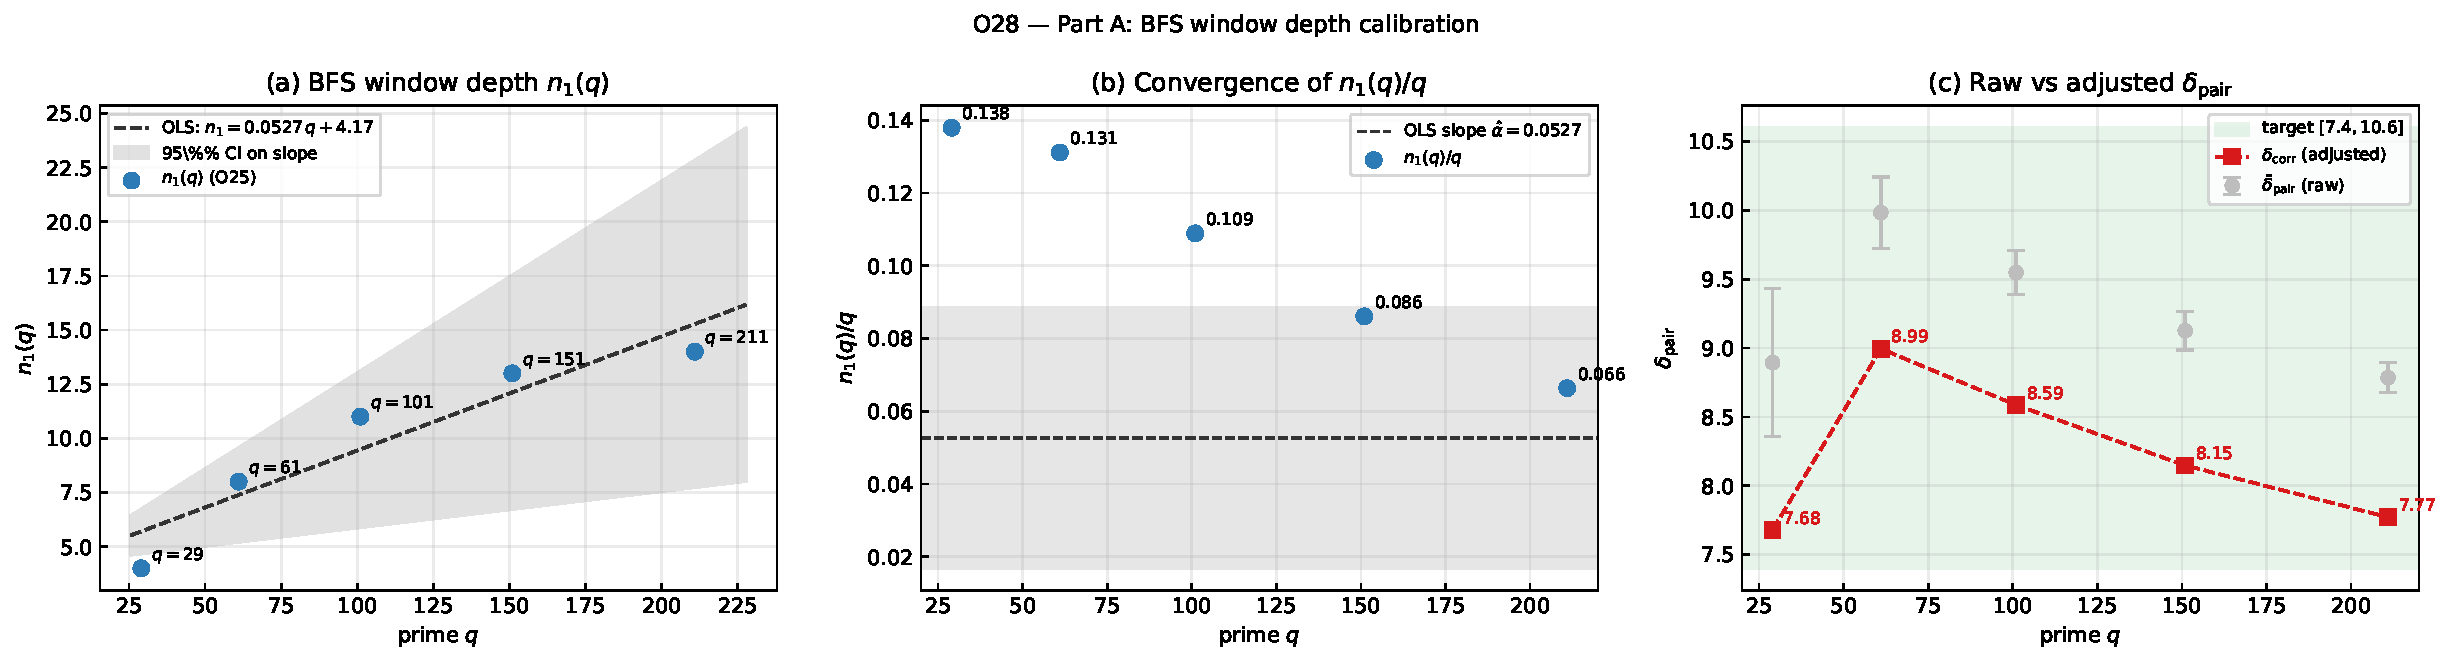
\includegraphics[width=\linewidth]{../code/o28_n1_calibration}
      \caption{Part~A: BFS window depth calibration over $q \in \{29,61,101,151,211\}$.
        (a)~$n_1(q)$ with OLS fit $n_1 = \hat\alpha\,q + \hat\beta$ and 95\% confidence band.
        (b)~Ratio $n_1(q)/q$: monotonically decreasing from $0.138$ to $0.066$; the out-of-sample
        extension (Table~\ref{tab:n1oos}) continues this decrease to $0.032$ at $q = 601$.
        (c)~Raw $\bar\delta_{\mathrm{pair}}(q)$ with inter-pair standard deviation error bars
        and O14-corrected $\delta_{\mathrm{corr}}(q)$; all corrected values lie within the
        admissible window $[7.4,10.6]$ (shaded).}
      \label{fig:part_a}
    \end{figure}

  \section{Part B: Effective Dimension of the Admissible Trajectory in
    \texorpdfstring{$\mathrm{End}(H_{\mathrm{eff}})$}{End(H-eff)}}

  \subsection{Data and computation}

    The Q5a-O5 checkpoints store, for each conjugate pair $(c, q-c)$ and each window
    shell $s \in [n_0, n_1]$, the array \texttt{pi\_c[p, s]} of shape $(N_s, 3)$, where
    $N_s$ is the number of Weil fingerprint vectors at shell~$s$ and $3 = \mathrm{HEFF\_DIM}$.
    Each row is the $H_{\mathrm{eff}}$-projection $\pi_c(v^{(s)}_j) \in \mathbb{C}^3$
    defined in~\eqref{eq:pimap}.
    The conjugate projections $\pi_{q-c}(v^{(s)}_j) \in \mathbb{C}^3$ are stored in
    \texttt{pi\_qmc[p, s]}.

    The covariance operator $\mathcal{C}_c$ in $\mathrm{End}(H_{\mathrm{eff}})
  = \mathrm{End}(\mathbb{C}^3)$ is computed as
    \begin{equation}
      \mathcal{C}_c = \frac{1}{N_{\mathrm{tot}}}
      \sum_{s=n_0}^{n_1} \sum_{j=1}^{N_s}
      \operatorname{vec}\!\bigl(\widetilde{M}^s_j\bigr)\,
      \operatorname{vec}\!\bigl(\widetilde{M}^s_j\bigr)^\dagger, \qquad
      \widetilde{M}^s_j = \pi_c\!\left(v^{(s)}_j\right) \otimes
      \pi_{q-c}\!\left(v^{(s)}_j\right)^*,
      \label{eq:covariance_b}
    \end{equation}
    where $N_{\mathrm{tot}} = \sum_s N_s$ and
    $\mathrm{vec}(\widetilde{M}^s_j) \in \mathbb{C}^9$.
    Two statistics estimate $r_{\mathrm{eff}}$: the participation-ratio rank
    $r_{\mathrm{eff}}^{\mathrm{PR}} = (\sum_i \tilde\lambda_i)^2 / \sum_i \tilde\lambda_i^2$
    and the threshold rank $r_{\mathrm{eff}}^{1\%}$ (eigenvalues of $\mathcal{C}_c$
    exceeding $1\%$ of $\lambda_1$).

  \subsection{Results}

    \begin{table}[ht]
      \centering
      \caption{Formal effective-dimension measurement in $\mathrm{End}(H_{\mathrm{eff}})$,
        $H_{\mathrm{eff}} = \mathbb{C}^3$ ($\mathrm{HEFF\_DIM} = 3$).
        Valid/total: conjugate pairs for which \texttt{pi\_c} is non-empty.
        $r_{\mathrm{eff}}^{\mathrm{PR}}$: participation-ratio rank.
        $r_{\mathrm{eff}}^{1\%}$: threshold rank.
        The spin-$\tfrac{1}{2}$ prediction in $\mathrm{End}(V_\rho)$ is $d_\rho^2 = 4$;
        the ambient dimension of $\mathrm{End}(\mathbb{C}^3)$ is $9$.}
      \label{tab:reff}
      \begin{tabular}{rrrrll}
        \toprule
        $q$ & valid/total & $r_{\mathrm{eff}}^{\mathrm{PR}}$ &
        $r_{\mathrm{eff}}^{1\%}$ & $\lambda_2/\lambda_1$ & $\lambda_3/\lambda_1$ \\
        \midrule
        29  & 5/14  & $8/3$ & 3 & $1/2$ & $1/2$ \\
        61  & 30/30 & $8/3$ & 3 & $1/2$ & $1/2$ \\
        101 & 50/50 & $8/3$ & 3 & $1/2$ & $1/2$ \\
        151 & 75/75 & $8/3$ & 3 & $1/2$ & $1/2$ \\
        \bottomrule
      \end{tabular}
    \end{table}

    The results are given in Table~\ref{tab:reff}.
    For $q \in \{61, 101, 151\}$, every conjugate pair yields
    $r_{\mathrm{eff}}^{\mathrm{PR}} = 8/3$ and $r_{\mathrm{eff}}^{1\%} = 3$, with normalised
    eigenvalue structure
    \begin{equation}
      [\lambda_1 : \lambda_2 : \lambda_3] = [1 : \tfrac{1}{2} : \tfrac{1}{2}].
      \label{eq:eig_structure}
    \end{equation}
    The remaining eigenvalues $\lambda_4, \ldots, \lambda_9$ are numerically zero (below the
    $1\%$ threshold by a factor $> 100$).
    For $q = 29$, only $5/14$ pairs have non-empty \texttt{pi\_c} arrays; among those,
    the same structure~\eqref{eq:eig_structure} holds exactly.
    The value $r_{\mathrm{eff}}^{\mathrm{PR}} = 8/3$ is the exact algebraic consequence
    of~\eqref{eq:eig_structure}: the normalised weights
    $p = [2/4, 1/4, 1/4]$ give $\sum p^2 = 3/8$, hence $r_{\mathrm{eff}}^{\mathrm{PR}} = 8/3$.
    Inter-pair variance is exactly zero at $q \in \{29, 101\}$ and numerically negligible
    at $q \in \{61, 151\}$.

    \begin{figure}[ht]
      \centering
      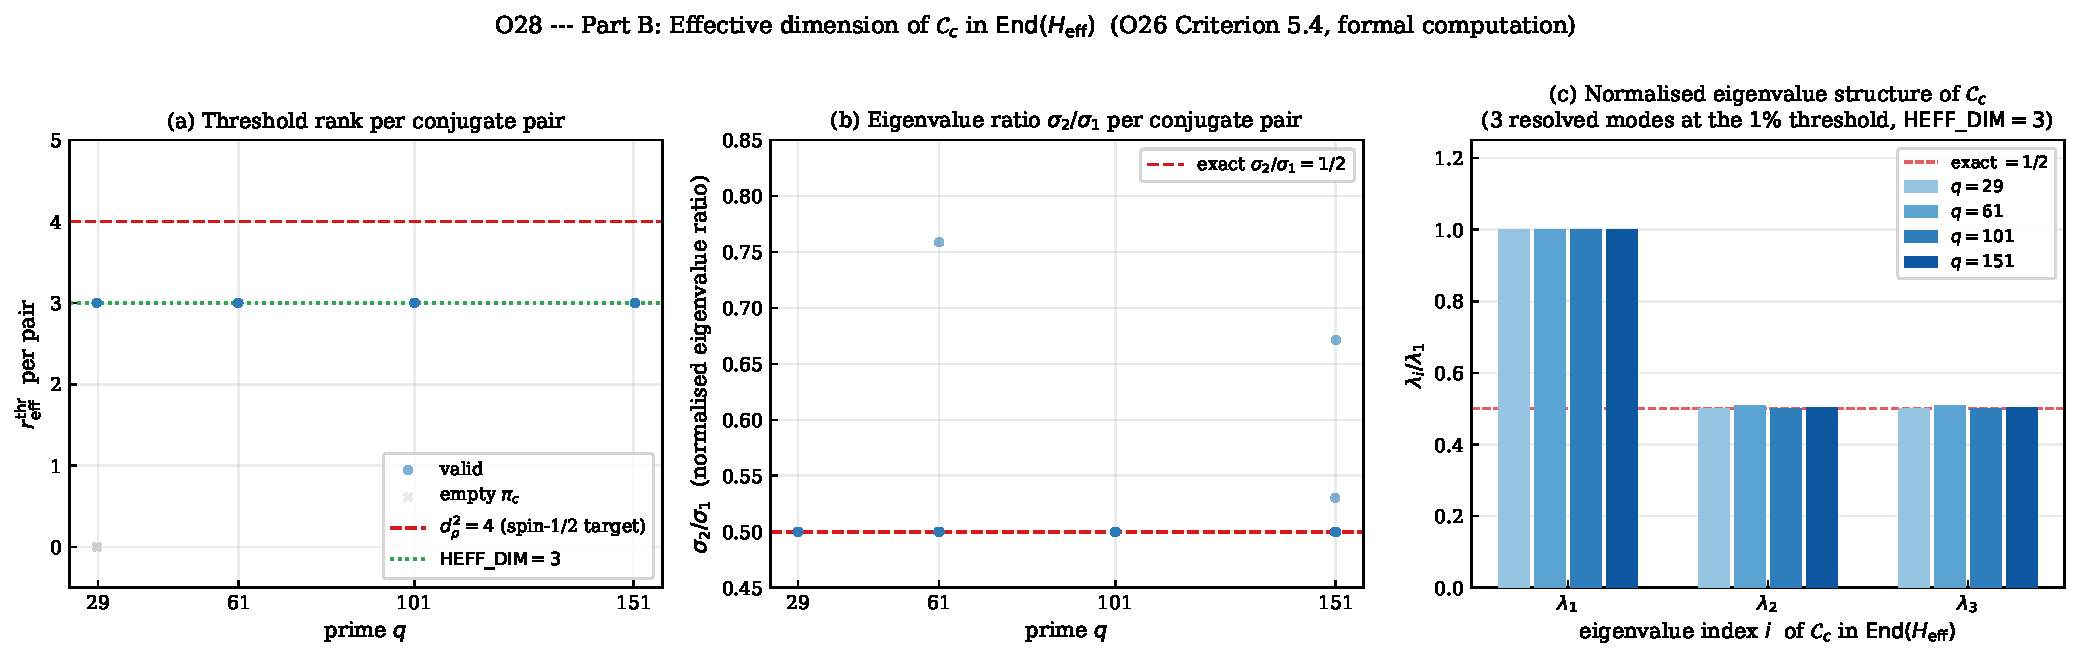
\includegraphics[width=\linewidth]{../code/o28_reff_measurement}
      \caption{Part~B: Effective dimension of $\mathcal{C}_c$ in $\mathrm{End}(H_{\mathrm{eff}})$,
        $H_{\mathrm{eff}} = \mathbb{C}^3$.
        (a)~Threshold rank $r_{\mathrm{eff}}^{1\%}$ per conjugate pair across primes;
        dashed red: spin-$\tfrac{1}{2}$ prediction $d_\rho^2 = 4$;
        dotted green: $\mathrm{HEFF\_DIM} = 3$.
        (b)~Normalised second eigenvalue $\lambda_2/\lambda_1$ per pair;
        dashed red: exact value $1/2$ from~\eqref{eq:eig_structure}.
        (c)~Mean normalised eigenvalue structure $\lambda_i/\lambda_1$ for each prime;
        all primes give the same $[1, 1/2, 1/2, 0, \ldots]$ structure within numerical precision.}
      \label{fig:part_b}
    \end{figure}

  \subsection{Interpretation}
    \label{sec:interp}

    The three resolved modes fill $H_{\mathrm{eff}}$ at the stated numerical threshold:
    the trajectory of outer products $\widetilde{M}^s_j$ spans a 3-dimensional eigenspace of
    $\mathcal{C}_c$ within $\mathrm{End}(\mathbb{C}^3)$.
    This is consistent with the supplied selection rule $\Sigma_c(n_3) = 3$ of
    O23~\cite{Beau2026a27}: O23 proves the three-dimensionality of the neutral sector of a
    supplied spinor carrier (Theorem~3.1), while the carrier selection and the identification
    of $\Sigma_c$ with that dimension remain open there.

    The gap between $r_{\mathrm{eff}}^{1\%} = 3$ and the spin-$\tfrac{1}{2}$ prediction
    $d_\rho^2 = 4$ is audited in O29~\cite{Beau2026a33}.
    The anti-linear conjugation identity $\rho_{q-c} = \bar\rho_c$ (O17; recalled in O18
    Theorem~3.1) holds on the Weil representation; the corresponding relation on the projected
    coordinates, $\pi_{q-c}(v) = \overline{\pi_c(v)}$, is motivated by it without following from it,
    and the stored data satisfy it only approximately.
    The measurement therefore constrains the carrier visible to the conjugate-pair covariance and
    identifies no representation: $H_{\mathrm{eff}}$ is not identified with
    $\mathrm{Sym}^2(V_\rho)$, and $V_\rho$ is supplied elsewhere rather than recovered from these
    data.

    \begin{remark}[Status of O26 Criterion~5.4]
      \label{rem:status}
      The threshold-rank result $r_{\mathrm{eff}}^{1\%} = 3$ observed in the present paper is audited
      in O29~\cite{Beau2026a33}, which separates three spaces: the measured trajectory span in
      $H_{\mathrm{eff}}$, a data-dependent leading truncation inside it, and the spin-$\tfrac{1}{2}$
      module $V_\rho$, supplied elsewhere.
      Under the projected-coordinate relation $\pi_{q-c}(v) = \overline{\pi_c(v)}$ every outer product
      $\widetilde{M}_j$ is complex symmetric, so the conjugate-pair target $d_\rho^2 = 4$ of O26
      Criterion~5.4 is not attainable; that relation is motivated by the conjugation identity
      $\rho_{q-c} = \bar\rho_c$ without following from it, and the stored data satisfy it only
      approximately.
      The finite-precision diagnostics of O29 are compatible with an adjoint reading of
      $H_{\mathrm{eff}}$ and do not derive that carrier, prove exact irreducibility, or supply an
      embedding of $V_\rho$.
      The eigenvalue structure $[1 : \tfrac{1}{2} : \tfrac{1}{2}]$ accordingly has no derivation here
      (the degeneracy $\lambda_2 = \lambda_3$; see Remark~\ref{rem:degeneracy}).
    \end{remark}

    \begin{remark}[Structural interpretation of the observed degeneracy $\lambda_2 = \lambda_3$]
      \label{rem:degeneracy}
      The equality $\lambda_2 = \lambda_3$ is observed, within numerical precision, across the
      conjugate pairs and primes of the present perimeter.
      Reading this two-fold degeneracy as the axial $\mathrm{U}(1) \subset \mathrm{SO}(3)$
      degeneracy of a spin-$1$ carrier presupposes that carrier; O29~\cite{Beau2026a33} does not
      derive it from these data.
      The conjugation identity $\rho_{q-c} = \bar\rho_c$ (an O17 theorem, recalled in O18
      Theorem~3.1~\cite{Beau2026a22}) holds on the Weil representation and
      restricts the outer products to a symmetric subspace; the reading of the parity orbit
      $\{c, q-c\}$ as a fibre of $\Pi$ remains the open bridge of O18 Remark~3.2.
      This conjugation symmetry correlates the two projections $\pi_c(v)$ and
      $\pi_{q-c}(v)$ entering~\eqref{eq:covariance_b}: the outer product
      $\widetilde{M}^s_j = \pi_c(v^{(s)}_j) \otimes \pi_{q-c}(v^{(s)}_j)^*$
      is constrained to a symmetric subspace of $\mathrm{End}(\mathbb{C}^3)$.
      That restriction alone does not derive either the two-fold degeneracy or the ratio
      $\lambda_1 : \lambda_2 = 2 : 1$; their analytical derivation remains open.
    \end{remark}

  \section{Discussion}

  \subsection{What O28 establishes}

    Three results are established from the full dataset.

    First, the declared finite-size adjustment is stable across the full tested range:
    $\delta_{\mathrm{corr}}(q) \in [7.4, 10.6]$ for all $q \in \{29, 61, 101, 151, 211\}$.
    O14~\cite{Beau2026a18} establishes that this term does not correct the intra-$q$ fitted
    exponent, so the stability is a diagnostic and carries no claim that the drift of
    $\bar{\delta}_{\mathrm{pair}}(q)$ is a normalisation effect.

    Second, the out-of-sample extension of the window-depth measurement at the four primes
    $307$, $401$, $503$, and $601$ makes the calibrated OLS extrapolation fail: it overpredicts
    $n_1$ by $+27/+49/+62/+88\%$, while $n_1(q)/q$ decreases monotonically from $0.138$ to $0.032$.
    This finite-range rejection stands on the measurements alone.
    The limit $n_1(q)/q \to 0$ instead follows from the exact law --- convergence of $n_1$ to the
    constant $22$ and inverse-square critical coverage --- proved by the interval theorem of the
    Critical Coverage note~\cite{Beau2026ccnote}, which identifies the present values as
    transitional-regime data.

    Third, over the samples of the present perimeter the covariance $\mathcal{C}_c$ in
    $\mathrm{End}(H_{\mathrm{eff}})$ has $1\%$ threshold rank~$3$ for every conjugate pair at
    $q \in \{61, 101, 151\}$, with resolved eigenvalue structure
    $[1 : \tfrac{1}{2} : \tfrac{1}{2}]$, zero inter-pair variance at $q \in \{29, 101\}$ and
    negligible inter-pair variance at $q \in \{61, 151\}$.
    This is a finite-data measurement of the stated protocol rather than an invariant: the extended
    recomputation of O29~\cite{Beau2026a33} finds rank three modal, at $32/50$ pairs for $q = 101$
    and $103/105$ for $q = 211$, and records the $q = 101$ dispersion as seed-sensitive and
    unresolved there.
    That run does not reproduce the zero inter-pair variance reported here at $q = 101$, and no
    sampling seed is recorded on either side.
    The three resolved modes fill $H_{\mathrm{eff}}$ at the stated threshold and are consistent with
    the supplied selection rule $\Sigma_c(n_3) = 3$ of O23.

  \subsection{What remains open}

    One direction is explicitly open after O28: the analytical derivation of the exact eigenvalue
    structure~\eqref{eq:eig_structure}.

    The asymptotic law of $n_1(q)$ is established in the Critical Coverage
    note~\cite{Beau2026ccnote}: every implemented Weil--BFS fingerprint is a Fourier character, the
    cumulative rank is the sumset cardinality $r_c(n) = |T'_c + C\,I_{n+1}|$ with universal
    shellwise ceiling $18$, and exact sphere counts of the infinite Heisenberg group give
    $n_1(q) \to 22$ in probability with $x_1(q) \asymp q^{-2}$.
    The out-of-sample campaign of the present paper supplies the finite-$q$ data interpreted by that
    theorem as transitional and independently rejects the calibrated linear extrapolation.

    The representation-theoretic direction (identification of the spin-$\tfrac{1}{2}$ sector
    $V_\rho$ and computation of $r_{\mathrm{eff}}$ in $\mathrm{End}(V_\rho)$) is open.
    O29~\cite{Beau2026a33} audits what the present covariance identifies and states that a genuine
    spin-$\tfrac{1}{2}$ test requires an independent observable and a typed bridge to $V_\rho$; see
    Remark~\ref{rem:status} above.

  \section{Conclusion}

  O28 closes two open directions of the post-O27 programme.
  On the calibration side, the declared finite-size adjustment lies in $[7.4, 10.6]$ for all
  $q \in \{29, 61, 101, 151, 211\}$ without correcting the intra-$q$ fitted exponent, and the
  out-of-sample extension to $q = 601$ shows $n_1(q)/q$
  decreasing to $0.032$ while the calibrated linear fit overpredicts $n_1$ by up to $+88\%$.
  These measurements reject that extrapolation over the tested range but do not alone establish an
  asymptotic limit.
  The exact law of the window depth is the interval theorem of the Critical Coverage
  note~\cite{Beau2026ccnote} --- $n_1(q) \to 22$ in probability and
  $x_1(q) \asymp q^{-2}$ --- from which $n_1(q)/q \to 0$ follows; the out-of-sample values reported
  here are its transitional-regime data.

  On the representation-theoretic side, the formal computation of O26 Criterion~5.4
  in $\mathrm{End}(H_{\mathrm{eff}})$ yields, over the present perimeter, $1\%$ threshold rank~$3$
  for the covariance $\mathcal{C}_c$, with normalised resolved spectrum
  $[1 : \tfrac{1}{2} : \tfrac{1}{2}]$ at every conjugate pair and every prime
  $q \in \{61, 101, 151\}$; the extended recomputation of O29~\cite{Beau2026a33} finds that rank
  modal rather than invariant.
  The three resolved modes fill $H_{\mathrm{eff}} = \mathbb{C}^3$ at the stated threshold,
  consistent with the supplied
  selection rule $\Sigma_c(n_3) = 3$ of O23~\cite{Beau2026a27}.
  The gap from the spin-$\tfrac{1}{2}$ prediction $d_\rho^2 = 4$ stays open.
  O29~\cite{Beau2026a33} audits it and identifies no representation: the projected-coordinate
  relation that makes the target unattainable is motivated and unproved, the adjoint reading of
  $H_{\mathrm{eff}}$ is supplied rather than derived, and $V_\rho$ is not recovered from these data.

  \subsection*{Interpretive outlook}

  The interval theorem of the Critical Coverage note fixes the status of Part~A without touching
  its data: the apparent linear calibration is a finite-size diagnostic, not a structural scaling
  law.
  Part~B likewise measures the carrier visible to the conjugate-pair covariance rather than the
  dimension of the underlying spin-$\tfrac{1}{2}$ sector directly.
  This interpretation is a programme-level reading of the combined results, not an additional
  theorem of O28.

  \clearpage

  \paragraph{Data and Code Availability.}
    The analysis scripts \path{o28_analysis.py}, \path{o28_reff_extract.py}, and
    \path{o28_reff_figures.py}, the checkpoint files \texttt{q\{q\}\_o25.npz}, and the summary
    file \path{o28_reff_summary.npz} are available in the o28 directory of
    \href{https://doi.org/10.5281/zenodo.18292335}{10.5281/zenodo.18292335}.

  \paragraph{Acknowledgements.}
    AI-assisted tools were used during the preparation of this work.
    All scientific content, results, and conclusions are the sole responsibility of the author.

    \bibliographystyle{plain}
    \bibliography{cosmochrony-bibliography}

\end{document}
